\newpage
\subsection{Conclusions}
The total uncertainty of the hygrometer obtained after including the calibration error and the hysteresis is $1.7$\%RH. For the array sensors the uncertainty is about $4\%$.
As the hygrometer design turned out to be more consistent and robust, it was also tested with the sniffing system and its ceramic sensor. The sensors array didn't provide expected repeatability and it need will be further tested inside the thermal demonstrator (see section~\ref{demo}). The design and the performance of the hygrometer was confirmed during the low temperature tests with the industrial capacitive sensors and with the trace humidity sensor (see figure~\ref{fig_comparison}). The uncertainties of the sensors were not shown, in order to represent the trends of the respective sensors. The largest uncertainty is associated with the capacitive sensor. 
\begin{figure}[!h]
\centering
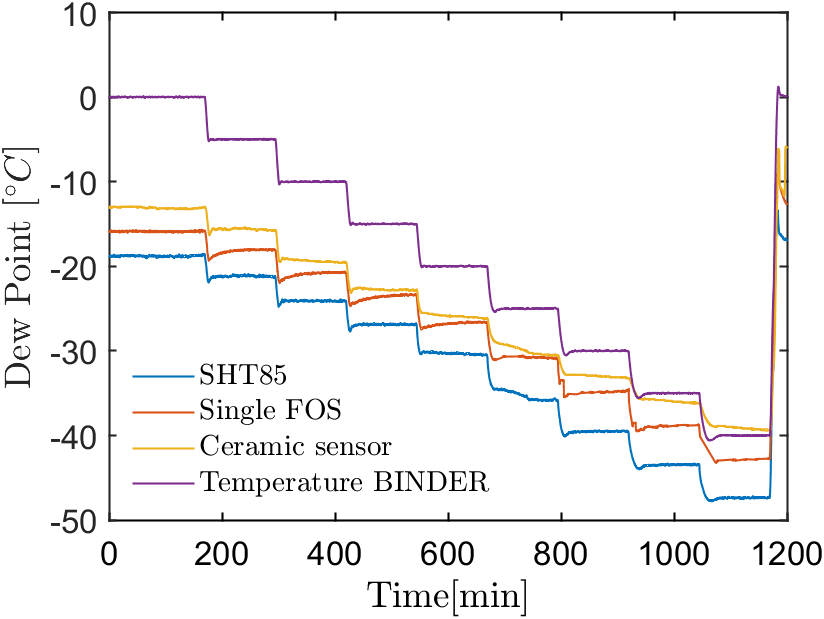
\includegraphics[width=0.6\columnwidth]{Chapter5/images/DPCPercent.png}
\caption{Comparison of the dew points calculated using Magnus formula for the industrial sensor SHT85, metal oxide trace humidity sensor and the hygrometer. For the comparison the temperature inside the Binder climatic chamber was also plotted.}
\label{fig_comparison}
\end{figure}
The response of the hygrometer was also compared with the sniffing system and different lengths of the guide lines leading to the ceramic sensor. In the case of the \gls{STS} the sniffing system's electronic circuitry will be placed at least \SI{20}{\metre} away from the detector. For plot depicted on the left side the pipe was \SI{2}{\metre} and for the right one \SI{12}{\metre}, the time response was $1.5$~min and $3$~m. Assuming that the flow doesn't depend on the distance from the sniffing point, if the pipe was $30$~m the response would be $5.7$~min. 
\begin{figure}[!h]
\centering
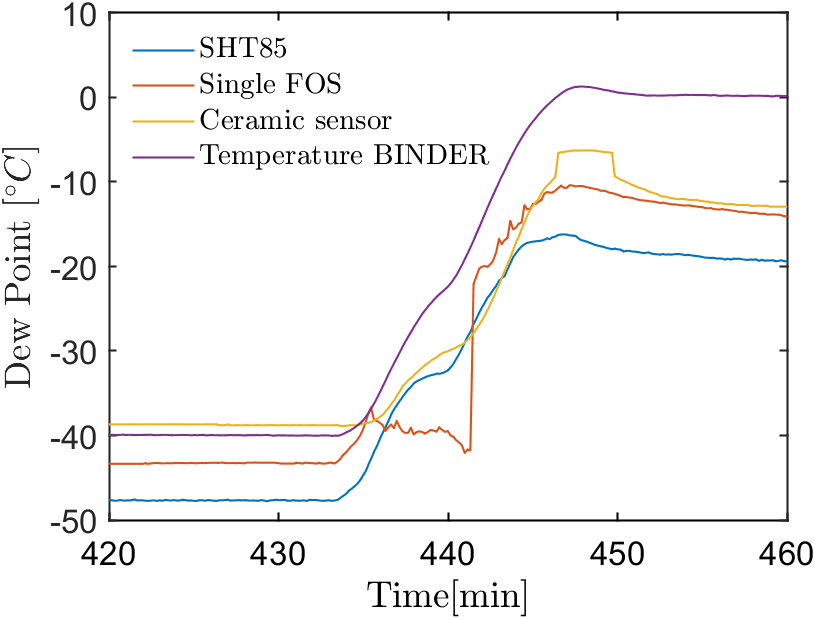
\includegraphics[width=0.47\columnwidth]{Chapter5/images/DPCPercent_response2m.png}
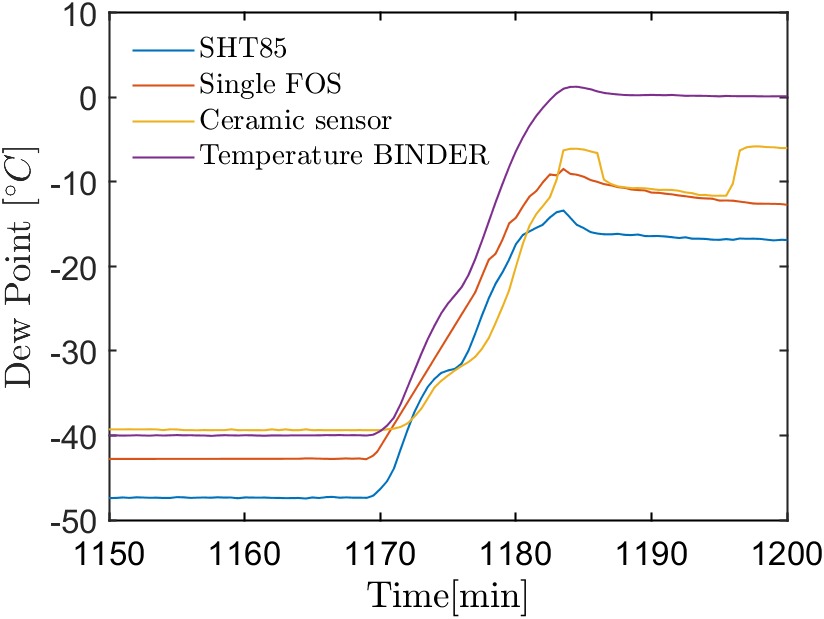
\includegraphics[width=0.47\columnwidth]{Chapter5/images/DPCPercent_response12m.png}
\caption{Time response comparison of different sensors. Left - \SI{2}{\metre} pipe to the ceramic sensors, right - \SI{12}{\metre} pipe to the ceramic sensors.}
\label{fig_comparison}
\end{figure}
\newpage
Figure \ref{Tfig_comparison_2} shows the behavior of the fiber optic hygrometer at low dew points. The sensing limits are clearly represented on the figure~\ref{Tfig_comparison_2} with a red rectangle. Considering the area with a high points density, the limitations of the hygrometer could be assumed to be a dew point of \SI{-70}{\celsius}. But in that area the uncertainties become much higher. It's also noteworthy that that limit refers to the measuring temperature of \SI{10}{\celsius}. On the other hand, for the dew points measured at \SI{20}{\celsius} the range shrinks to values of about \SI{-50}{\celsius}/\SI{-40}{\celsius}.

\begin{figure}[!h]
\centering
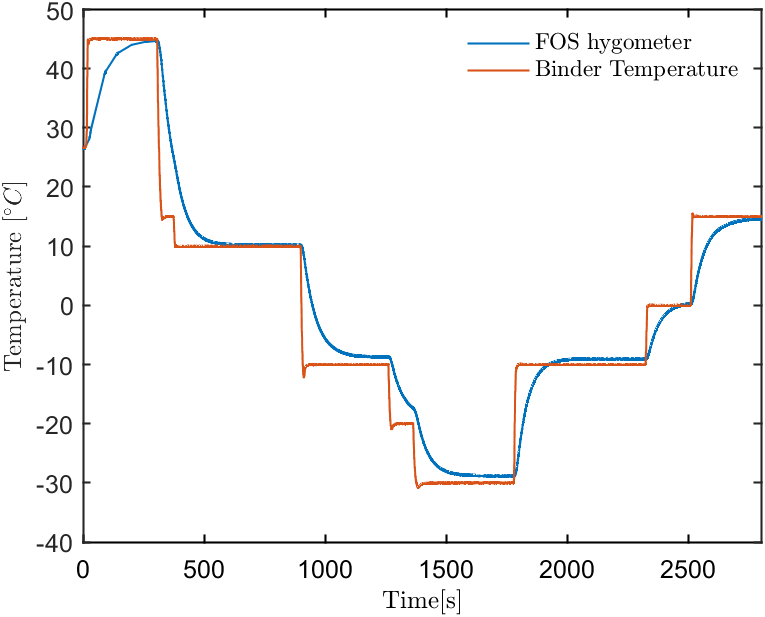
\includegraphics[width=0.47\columnwidth]{Chapter5/images/FOS_performance_T.png}
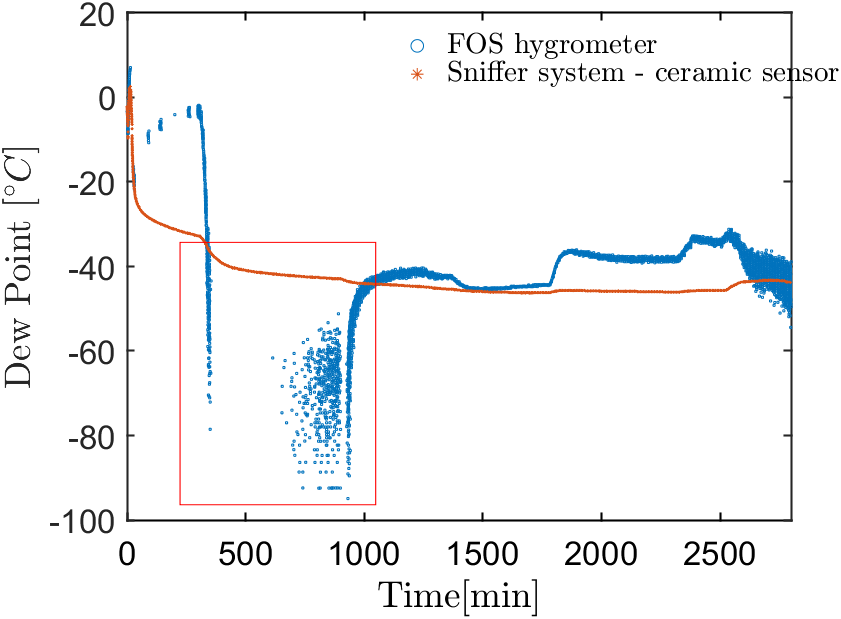
\includegraphics[width=0.47\columnwidth]{Chapter5/images/FOS_performance1.png}
\caption{The temperature inside the BINDER chamber and temperature measured by the hygrometer(left). Dew point during the changing ambient conditions per the hygrometer and the ceramic sensor}
\label{Tfig_comparison_2}
\end{figure}

\newpage
\section{Final considerations}
Such parameters, both for the \gls{FOS} and sniffing system, meet \gls{STS} requirements and will be most likely combined to form a distributed sensing system.


Three different sensor technologies will be measuring the ambient parameters: Fiber Optic Sensors (FOS FBG-based), commercially available capacitive sensors (SHT series), and a sniffing system based on trace humidity sensors.
Several sniffing points inside the detector enclosure will measure trace humidity and serve as a  reference for the two other measurement technologies. Moreover, the sniffing system is going to be the base for the interlock system, which will take action in case of hazardous humidity levels. In this contribution, we summarize efforts to choose, design, and characterize RH FBG FOS.